\documentclass[tikz, border=14pt]{standalone}
\usepackage{tikz}
\usepackage{mathtools}
\usetikzlibrary{bayesnet}
\begin{document}
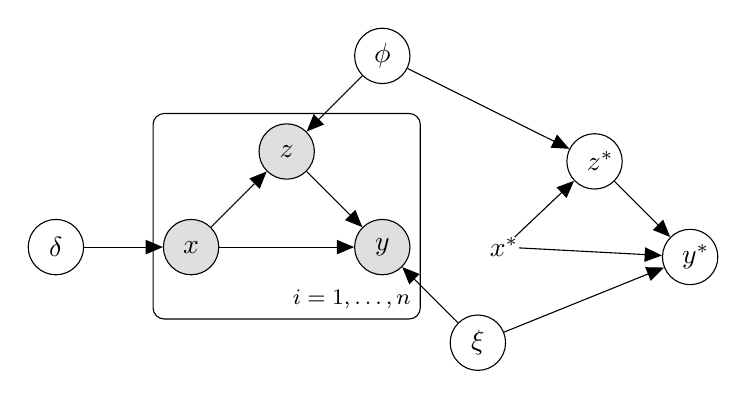
\begin{tikzpicture}
    \node[obs] (x) {$x$};
    \node[obs, above right = of x] (z) {$z$};
    \node[obs, below right = of z] (y) {$y$};
    \edge{x}{y};
    \edge{z}{y};
    \edge{x}{z};
    \plate {plate1} {(x)(y)(z)} {$i=1,\ldots, n$ };
    
    \node[const, right = of y] (x2) {$x^\ast$};
    \node[latent, above right = of x2] (z2) {$z^{\mathrlap{\ast}}$};
    \node[latent, below right = of z2] (y2) {$y^{\mathrlap{\ast}}$};
    \edge{x2}{y2};
    \edge{z2}{y2};
     \edge{x2}{z2};
        
    \node[latent, left = of x] (delta) {$\delta$}; 
    \node[latent, above right = of z] (phi) {$\phi$};
    \node[latent, below right = of y] (xi) {$\xi$};
    \edge{xi}{y,y2};
    \edge{phi}{z, z2};
    \edge{delta}{x};
\end{tikzpicture}
\end{document}